\documentclass[a4paper,11pt]{article}

% Identificação
\newcommand{\pbtitulo}{Guia para ESP32}
\newcommand{\pbversao}{1.1}

\usepackage{../sty/tutorial}

%----------------------------------------------------------------------
% Início do Documento
%----------------------------------------------------------------------
\begin{document}

\maketitle % mostrar o título
\thispagestyle{fancy} % habilitar o cabeçalho/rodapé das páginas

%-----------------------------------------------------------------------------
% RESUMO DO ARTIGO
%-----------------------------------------------------------------------------

\begin{abstract}
\initial{ESP32}\textbf{é um microcontrolador com baixo custo/consumo de energia que se tornou o queridinho absoluto para projetos de Internet das Coisas (IoT), automação residencial e prototipagem de hardware. Desenvolvido pela Espressif Systems, é o sucessor do famoso \textbf{ESP8266}, trazendo um salto gigante em processamento e conectividade.}
\end{abstract}

%-----------------------------------------------------------------------------
% CONTEÚDO DO ARTIGO
%-----------------------------------------------------------------------------
\section{Introdução}
A placa \textbf{ESP32} se destaca principalmente por sua capacidade de comunicação sem fio aliada ao poder de processamento, tornando-o extremamente versátil. A maior vantagem é ter Wi-Fi (802.11 b/g/n) e Bluetooth (v4.2 BR/EDR e BLE - \textit{Bluetooth Low Energy}) integrados no mesmo chip. Elimina a necessidade de módulos externos, isso permite que o projeto se conecte à rede local, envie dados para a nuvem ou se comunique diretamente com smartphones e outros sensores BLE.
\begin{figure}[H]
	\centering
	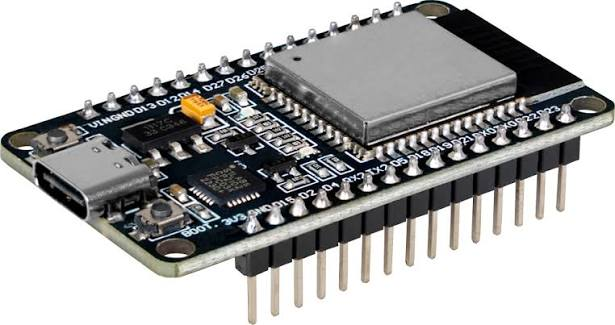
\includegraphics[width=0.5\textwidth]{imagens/esp32c.jpeg}
	\caption{Modelo ESP32-Classic}
\end{figure}

Outro ponto significativo, enquanto outras placas como \textbf{Arduino} que possuem processadores de 8 bits operando a 16 MHz, o ESP32 possui: \vspace{-1em}
\begin{itemize}
	\item Processador Dual-Core (Tensilica Xtensa 32-bit LX6).
	\item Frequência de clock de até 240 MHz.
	\item Memória RAM abundante: 520 KB de SRAM interna + suporte a PSRAM externa.
\end{itemize}

Apesar de toda a potência e recursos de conectividade, a placa de desenvolvimento do ESP32 possui um custo muito baixo no mercado, tornando-a acessível tanto para hobbystas quanto para aplicação em produtos comerciais.

ESP32 não fica preso a apenas uma linguagem ou ecossistema. Dependendo do foco do projeto (prototipagem rápida vs. firmware industrial), podemos programá-lo com: \vspace{-1em}
\begin{itemize}
	\item \textbf{Suporte a IDEs}: Pode ser programado diretamente pela Arduino IDE (C/C++), PlatformIO (VS Code) ou pelo framework oficial da fabricante, o ESP-IDF.
	\item \textbf{Linguagens alternativas}: Compatível com MicroPython e CircuitPython, ideal para rápida prototipagem.
	\item \textbf{Ainda aceita}: RUST (esp-rs/bare-metal), JavaScript/LUA (Kaluma/NodeMCU) ou YAML (ESPHome)
\end{itemize}

Arduino IDE / PlatformIO é a forma mais popular. Utiliza as bibliotecas tradicionais do Arduino com suporte direto às funções nativas e dual-core do ESP32. Perfeito para prototipagem rápida e projetos acadêmicos. Já o \textbf{ESP-IDF} (Espressif IoT Development Framework), é o SDK oficial mantido pela fabricante. Permite acesso direto ao sistema operacional em tempo real (FreeRTOS), controle fino de memória, otimização de baixo consumo e gerenciamento avançado de rede Wi-Fi e Bluetooth.

Observações a parte ficam por conta do MicroPython, que é uma implementação otimizada do Python 3 para microcontroladores. Executa diretamente no chip com um terminal interativo (REPL). Ideal para manipular estruturas de dados JSON, requisições HTTP/MQTT e lidar com lógica complexa em poucas linhas de código. E lembramos que a comunidade do ecossistema Rust vem crescendo bastante com a iniciativa esp-rs. Garante segurança de memória sem o \textit{Garbage Collector} e alta performance, adotado em novos projetos industriais onde travamentos por vazamento de memória não podem ocorrer.

\section{Guia das Placas Oficiais Disponíveis}
A \textbf{Espressif} (fabricante do ESP32) diversificou a linha criando várias famílias de placas. Cada uma foi projetada para atender a um propósito de mercado específico, equilibra custo, consumo de energia, capacidade de processamento e recursos de conectividade.

\begin{figure}[H]
	\centering
	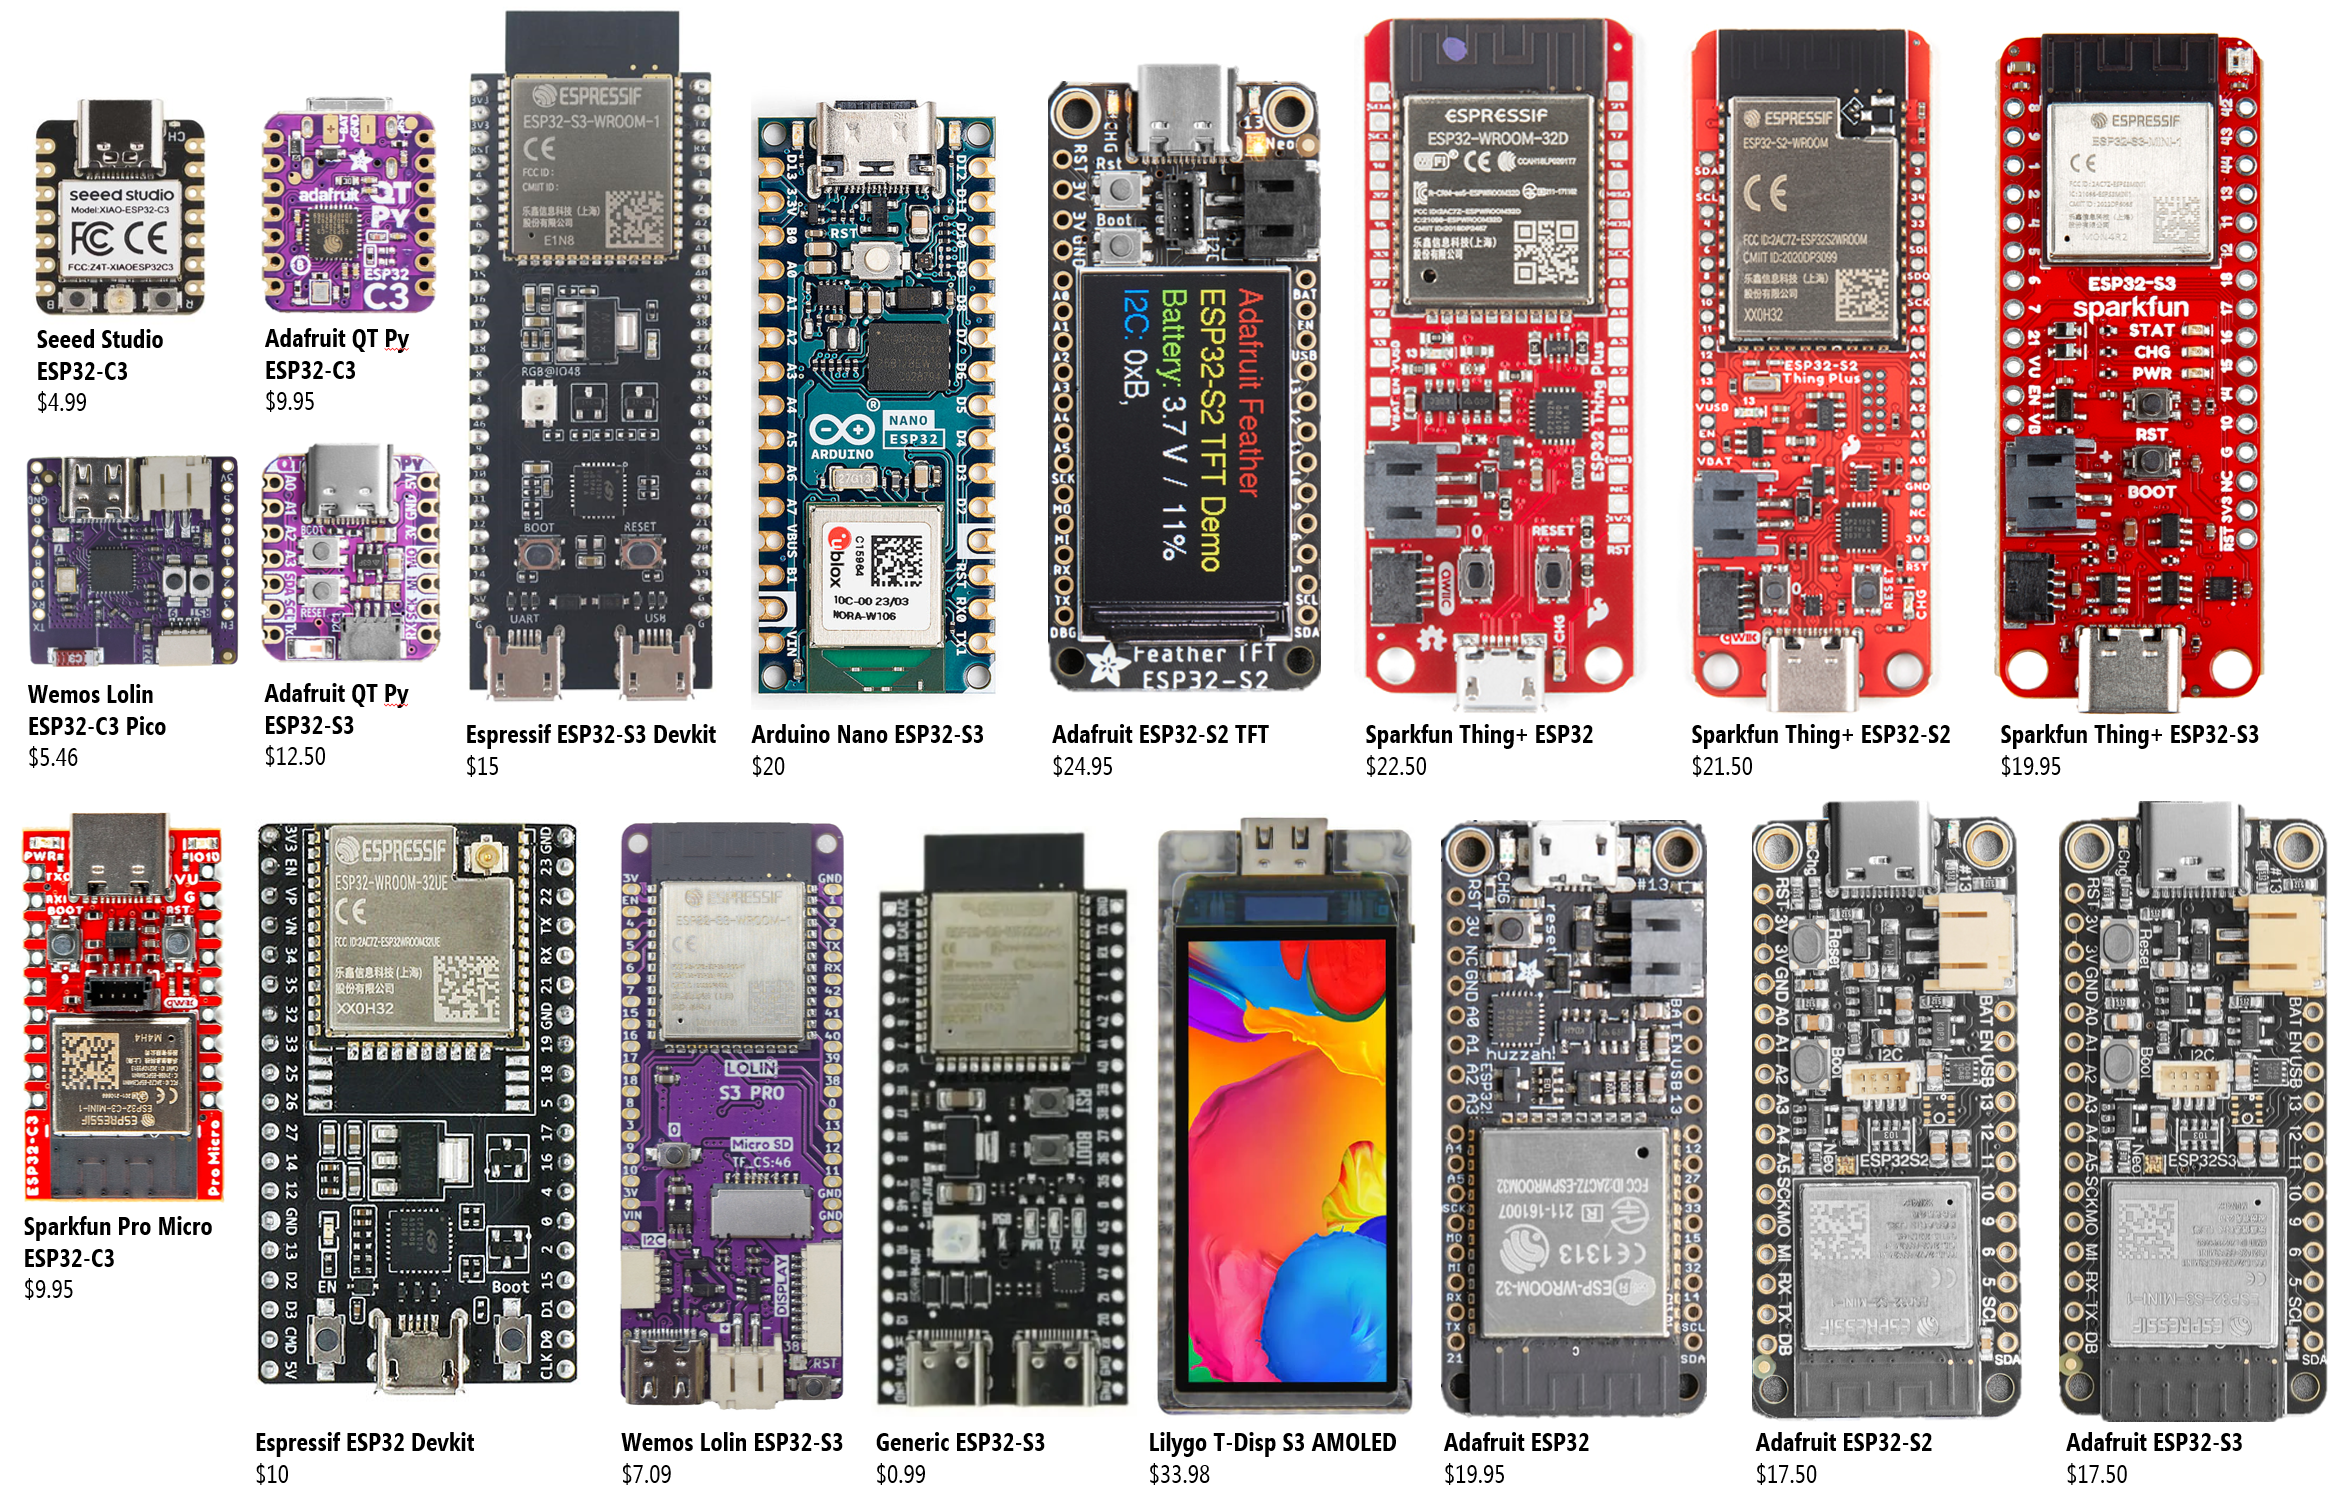
\includegraphics[width=0.6\textwidth]{imagens/familiaEsp.png}
	\caption{Família do ESP32 com preços médio em Dólar}
\end{figure}

ESP32 se estabeleceu como a solução definitiva para o desenvolvimento de sistemas embarcados e \textbf{Internet das Coisas} (IoT) graças ao seu equilíbrio ímpar entre alto desempenho e baixo custo. Ao integrar conectividade \textbf{Wi-Fi} e \textbf{Bluetooth} nativas em uma placa de processamento poderoso -- que chega a oferecer até dois núcleos operando a 240 MHz --, a plataforma elimina a necessidade de módulos externos complexos. Porém para utilizá-lo com segurança, e não gastar dinheiro a toa, preparei esse guia que pode lhe auxiliar quando pensar em adquirir uma (ou várias) dessas placas.

\subsection{ESP32 Clássico (O "Original")}
\textbf{Dados Técnicos}: \vspace{-1em}
\begin{itemize}[nolistsep]
	\item Conectividade Sem Fio	com Wi-Fi 4 (2.4 GHz)
	\item Bluetooth Classic com BLE 4.2
	\item Dual-Core Xtensa LX6 (com até 240 MHz CPU)
	\item Memória SRAM de 520 Kb 
\end{itemize}

\textbf{Motivo da existência}: Suprir a necessidade de uma placa de baixo custo com alto poder de processamento dual-core e conectividade dupla (Wi-Fi + Bluetooth BR/EDR/BLE) nativa.

\textbf{Problemas}: \vspace{-1em}
\begin{itemize}[nolistsep]
	\item Somente se utiliza do \textit{Bluetooth Classic}
	\item \textit{Sensor Hall}\footnote{Um sensor Hall (ou sensor de efeito Hall) é um dispositivo eletrônico que serve para detectar e medir campos magnéticos. Ele funciona gerando um sinal de tensão elétrica sempre que se aproxima de um ímã.} está depreciado
	\item Baixo nível de segurança
\end{itemize}

Para que serve: Projetos genéricos, automação residencial e prototipagem que exigem multitarefa.  

\subsection{Série ESP32-S (Foco em Desempenho, Telas, USB e IA)}
\textbf{Motivo da existência}: Atender aplicações que exigem processamento gráfico, controle direto por USB, conectividade de câmera/áudio e inteligência artificial na borda (Edge AI).  

\textbf{Principais modelos}:

\textbf{ESP32-S2}: Uma opção single-core focada em suporte a USB nativo (USB OTG) e segurança reforçada, descartando o Bluetooth para baratear.  

\textbf{Dados Técnicos}: \vspace{-1em}
\begin{itemize}[nolistsep]
	\item Conectividade Sem Fio	com Wi-Fi 4 (2.4 GHz)
	\item Single-Core Xtensa LX7 (com até 240 MHz CPU)
	\item Memória SRAM de 320 Kb
	\item Full-Speed USB-OTG
\end{itemize}

\textbf{Problemas}: \vspace{-1em}
\begin{itemize}[nolistsep]
	\item Extremamente simplificada
	\item Sem conexão Bluetooth
	\item Sem MCPWM\footnote{\textbf{MCPWM} sigla para \textit{Motor Control Pulse Width Modulator} (Modulador de Largura de Pulso para Controle de Motor). É um periférico de hardware especializado em microcontroladores (como o ESP32) projetado para gerar sinais de controle avançados para motores elétricos e fontes de energia.}
\end{itemize}

\textbf{ESP32-S3}: Essa placa é o carro-chefe em desempenho. Traz dois núcleos com instruções vetoriais para acelerar algoritmos de IA/reconhecimento de voz, mais pinos para displays LCD, câmeras (ESP32-CAM) e USB nativo.  

\textbf{Dados Técnicos}: \vspace{-1em}
\begin{itemize}[nolistsep]
	\item Conectividade Sem Fio	com Wi-Fi 4 (2.4 GHz) e BLE 5.0
	\item Dual-Core Xtensa LX7 (com até 240 MHz CPU)
	\item Memória SRAM de 512 Kb
	\item Full-Speed USB-OTG
	\item Suporte a Câmeras ou Telas LCD
\end{itemize}

\textbf{Problemas}: \vspace{-1em}
\begin{itemize}[nolistsep]
	\item Oferece somente suporte para Wi-Fi 4 (descarta Wi-Fi 6)
	\item Sem suporte a Bluetooth ou Rede
	\item Xtensa - Sem o RISC-V
\end{itemize}

\subsection{Série ESP32-C (Foco em Custo, Baixo Consumo e Padrão RISC-V)}
\textbf{Motivo da existência}: Substituir o antigo e simples ESP8266 por uma arquitetura aberta (RISC-V), focando em custo super baixo, economia de bateria e pinagem simplificada para dispositivos massivos de Casa Inteligente.

\textbf{Principais modelos}:

\textbf{ESP32-C2}: Sendo a placa mais barata de toda a família (podemos anotar que foi a real sucessora da \textbf{ESP8266}), possui suas dimensões reduzidas para aplicações de Internet das Coisas (IoT) extremamente simples e produzidas em larga escala. É a escolha ideal para substituir microcontroladores legados de 8 bits em lâmpadas inteligentes, sensores de porta/janela, tomadas conectadas e pequenos eletrodomésticos que necessitam apenas de conectividade básica e confiável.

\textbf{Dados Técnicos}: \vspace{-1em}
\begin{itemize}[nolistsep]
	\item Conectividade Sem Fio	com Wi-Fi 4 (2.4 GHz) e BLE 5.0
	\item Single-Core RISC-V (com até 120 MHz CPU)
	\item Memória SRAM de 272 Kb
\end{itemize}

\textbf{Problemas}: \vspace{-1em}
\begin{itemize}[nolistsep]
	\item Oferece somente 14 GPIOs\footnote{GPIO (\textit{General-Purpose Input/Output}), ou Entrada/Saída de Propósito Geral, são pinos programáveis encontrados em microcontroladores e microprocessadores. Servem como uma ponte de comunicação entre o chip e o mundo externo, permitindo enviar (saída) ou receber (entrada) sinais elétricos para controlar componentes ou ler sensores.}
	\item Memória muito limitada
	\item Sem inteface USB integrada
\end{itemize}

\textbf{ESP32-C3}: Placa compacta de núcleo único (entry-level) com Wi-Fi e Bluetooth 5 (BLE), feito para sensores simples, lâmpadas e tomadas inteligentes que não precisam de muito processamento.

\textbf{Dados Técnicos}: \vspace{-1em}
\begin{itemize}[nolistsep]
	\item Conectividade Sem Fio	com Wi-Fi 4 (2.4 GHz) e BLE 5.0
	\item Single-Core RISC-V (com até 160 MHz CPU)
	\item Memória SRAM de 400 Kb
\end{itemize}

\textbf{Problemas}: \vspace{-1em}
\begin{itemize}[nolistsep]
	\item Oferece único núcleo
	\item Sem suporte a USB OTG
	\item Somente com WiFi 4 - Sem Wi-Fi 6
\end{itemize}

\textbf{ESP32-C5}: Foi a primeira placa da marca a introduzir conectividade Wi-Fi 6 Dual-Band (operando tanto em 2.4 GHz quanto em 5 GHz - único da família), superando o gargalo de interferência e saturação das redes sem fio tradicionais.

\textbf{Dados Técnicos}: \vspace{-1em}
\begin{itemize}[nolistsep]
	\item Conectividade Sem Fio	com Wi-Fi 6 (2.4 GHz + 5 GHz) e BLE 5.0
	\item Single-Core RISC-V (com até 240 MHz CPU)
	\item Memória SRAM de 400 Kb
	\item Suporte a 802.15.4 (Zigbee/Thread)
	\item Suporte ao \textbf{Matter}\footnote{\textbf{Matter} é um padrão universal de conexão para casas inteligentes. Isso quer dizer que o dispositivo pode conversar com produtos de outras marcas e funcionar em vários aplicativos sem problemas como Apple, Google, Amazon e Samsung.}
\end{itemize}

\textbf{Problemas}: \vspace{-1em}
\begin{itemize}[nolistsep]
	\item Oferece único núcleo
	\item Mínimo suporte a \textit{firmware} (novo device)
	\item Placa com uma seleção limitada
\end{itemize}

\textbf{ESP32-C6}: Criado para suportar protocolos modernos como Wi-Fi 6, Zigbee e Thread (padrão Matter), garantindo relevância no ecossistema moderno de casa inteligente.  

\textbf{Dados Técnicos}: \vspace{-1em}
\begin{itemize}[nolistsep]
	\item Conectividade Sem Fio	com Wi-Fi 6 (2.4 GHz) e BLE 5.3
	\item Single-Core RISC-V (com até 240 MHz CPU)
	\item Memória SRAM de 512 Kb
	\item Suporte a 802.15.4 (Zigbee/Thread)
	\item Suporte ao \textbf{Matter}
\end{itemize}

\textbf{Problemas}: \vspace{-1em}
\begin{itemize}[nolistsep]
	\item Oferece único núcleo
	\item Sem câmera ou interface de display
	\item Somente 2.4 GHz de banda
\end{itemize}

\textbf{ESP32-C61}: Uma alternativa ultra-otimizada e ainda mais acessível ao \textbf{ESP32-C6}, focando em entregar o essencial na conectividade IP direta com \textbf{Wi-Fi 6} (802.11ax na banda de 2.4 GHz) e do Bluetooth 5 (LE) com menor custo e tamanho. É a escolha ideal para dispositivos Wi-Fi 6 de baixo custo na casa inteligente (como tomadas, eletrodomésticos e hubs locais) que exigem maior capacidade de \textit{buffer} e atualizações de \textit{firmware} mais complexas.

\textbf{Dados Técnicos}: \vspace{-1em}
\begin{itemize}[nolistsep]
	\item Conectividade Sem Fio	com Wi-Fi 6 (2.4 GHz) e BLE 5.0
	\item Single-Core RISC-V (com até 160 MHz CPU)
	\item Memória SRAM de 256 Kb
\end{itemize}

\textbf{Problemas}: \vspace{-1em}
\begin{itemize}[nolistsep]
	\item Sem suporte a Zigbee ou Thread
	\item Baixa quantidade de GPIOs disponíveis, porém maior que o modelo C6.
	\item Um único núcleo de 160 MHz
\end{itemize}

Seu grande diferencial está na adição de suporte para \textbf{PSRAM} externa integrada e recursos reforçados de segurança (como criptografia de memória e \textbf{ECDSA}\footnote{ECDSA sigla para \textit{Elliptic Curve Digital Signature Algorithm} (Algoritmo de Assinatura Digital de Curva Elíptica). É um método criptográfico usado para criar e verificar assinaturas digitais, garante a autenticidade e a integridade de dados e mensagens na internet.}).

\subsection{Série ESP32-H (Foco Exclusivo em Redes Mesh / Zigbee)}
\textbf{Motivo da existência}: Atender aplicações que operam puramente com baterias e não precisam de Wi-Fi, mas exigem comunicação em malha (mesh) ultrarrápida e eficiente.

\textbf{ESP32-H2}: Não possui Wi-Fi. Traz apenas Bluetooth 5 e rádios para IEEE 802.15.4 (Zigbee e Thread/Matter), ideal para fechaduras, interruptores sem fio e sensores de presença acionados a pilha.

\textbf{Dados Técnicos}: \vspace{-1em}
\begin{itemize}[nolistsep]
	\item Conectividade Sem Fio	com BLE 5.0
	\item Single-Core RISC-V (com até 96 MHz CPU)
	\item Memória SRAM de 320 Kb
	\item Suporte a 802.15.4 (Zigbee/Thread)
	\item Suporte ao \textbf{Matter}
\end{itemize}

\textbf{Problemas}: \vspace{-1em}
\begin{itemize}[nolistsep]
	\item Sem Wi-Fi
	\item Baixa quantidade de GPIO disponíveis
	\item Um único núcleo de 160 MHz
\end{itemize}

\textbf{ESP32-H4}: Ultra-baixo consumo com foco em conectividade sem fio avançada e recursos de áudio e localização. Seu grande diferencial em relação ao H2 é a introdução do suporte a \textbf{LE Audio} (transmissão de áudio sem fio com baixo consumo), canais isócronos e tecnologias de goniometria/localização interna (AoA/AoD), além de um conversor DC-DC integrado para máxima economia de energia em baterias pequenas tipo moeda. Escolha ideal para novos \textit{wearables}\footnote{Wearables, ou tecnologias vestíveis, são dispositivos eletrônicos inteligentes projetados para serem usados diretamente no corpo como acessórios ou roupas. Exemplos mais comuns incluem relógios, pulseiras de atividade e anéis.}, dispositivos de saúde, acessórios de áudio sem fio e nós de sensores em redes \textbf{Matter} de grande escala operados a bateria.

\textbf{Dados Técnicos}: \vspace{-1em}
\begin{itemize}[nolistsep]
	\item Conectividade Sem Fio	com BLE 5.4
	\item Dual-Core RISC-V (com até 96 MHz CPU)
	\item Memória SRAM de 320 Kb
	\item Suporte a 802.15.4 (Zigbee/Thread)
	\item Suporte ao \textbf{Matter}
\end{itemize}

\textbf{Problemas}: \vspace{-1em}
\begin{itemize}[nolistsep]
	\item Sem Wi-Fi
	\item DevKits não são fáceis de localizar
	\item Velocidade do "\textit{Clock}" interno é somente 96 MHz
\end{itemize}

\subsection{Série ESP32-P (Foco em Computação de Alta Performance Sem Wi-Fi Nativo)}
\textbf{Motivo da existência}: Atender sistemas embarcados complexos e Interfaces Homem-Máquina (IHM) que necessitam de telas sensíveis ao toque com alta resolução, processamento de vídeo e várias portas de comunicação, sem focar na parte de rádio Wi-Fi.

\textbf{ESP32-P4}: Um chip dual-core RISC-V com clock alto (400 MHz), suporte avançado a codecs de vídeo/áudio e aceleradores de hardware.  

\textbf{Dados Técnicos}: \vspace{-1em}
\begin{itemize}[nolistsep]
	\item Dual-Core RISC-V (com até 400 MHz CPU)
	\item Memória SRAM de 748 Kb
	\item Suporte a câmeras, telas ou H.264\footnote{H.264 é um padrão de compressão de vídeo popular, também conhecido como AVC (Advanced Video Coding) ou MPEG-4 Parte 10. Utilizado para deixar arquivos de vídeo mais leves e fáceis de transmitir ou armazenar sem perder muita qualidade.}
\end{itemize}

\textbf{Problemas}: \vspace{-1em}
\begin{itemize}[nolistsep]
	\item Sem Wi-Fi
	\item DevKits não são fáceis de localizar
	\item Para Wireless verificar o suporte disponível
\end{itemize}

\subsection{Resumindo}
Então antes de correr para comprar uma placa, temos que pensar em qual projeto vamos montar: \vspace{-1em}
\begin{itemize}
	\item Clássico: Para o uso geral e prototipagem do dia a dia.
	\item Série S: Para telas, câmeras, USB nativo e Inteligência Artificial.  
	\item Série C: Para sensores simples, lâmpadas, conectividade em massa e baixo consumo.  
	\item Série H: Para automação alimentada por bateria rodando Zigbee/Matter.
	\item Série P: Para painéis gráficos complexos e IHM.
\end{itemize}

\section{Arduino Nano ESP32}
É o resultado da união oficial entre o ecossistema da \textbf{Arduino} e o poder de processamento sem fio da \textbf{Espressif}. Desenvolvido no tradicional e compacto fator de forma Nano (fácil de usar em protoboards), traz o chip ESP32-S3 (Dual-Core 32-bit LX7 até 240 MHz, com suporte a Wi-Fi de 2.4 GHz e Bluetooth 5 LE).

\begin{figure}[H]
	\centering
	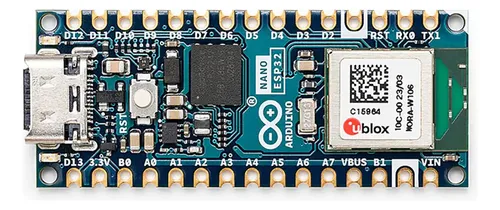
\includegraphics[width=0.6\textwidth]{imagens/ArduinoESP.png}
	\caption{Placa Arduino Nano ESP32}
\end{figure}

A grande vantagem desse modelo em relação às placas genéricas de ESP32 é a experiência do ecossistema Arduino: conta com suporte oficial ao pinout clássico do Arduino Nano, USB-C nativo (que facilita depuração e simulação de periféricos HID como teclado/mouse), suporte ao ecossistema Arduino Cloud para criação de dashboards IoT em minutos e compatibilidade nativa tanto para programação em C++ (Arduino IDE) quanto em MicroPython. É a escolha perfeita para quem quer a facilidade de uso do Arduino aliada ao alto desempenho, recursos gráficos/IA leves e conectividade do ESP32-S3 em um formato ultra-compacto.

 \vspace{-1em}
\begin{itemize}
	\item Microcontrolador: u-blox NORA-W106-10B (baseado no ESP32-S3)
	\item 32-bit Dual-Core Xtensa LX7 (até 240 MHz) com aceleradores vetoriais
	\item Memória Flash de16 MB (External Flash)
	\item Memória SRAM de 512 KB interna + 8 MB PSRAM externa
	\item Conectividade Sem Fio	Wi-Fi 4 (802.11 b/g/n a 2.4 GHz) + Bluetooth 5 (LE)
	\item USB-C (com suporte a USB OTG nativo)
\end{itemize}

Como o chip principal é um ESP32-S3, a porta USB-C é conectada diretamente ao silício do processador (sem chip conversor Serial-USB intermediário). Permite que a placa seja reconhecida pelo computador como teclado, mouse ou dispositivo MIDI nativo (USB HID), além de viabilizar a depuração de código em tempo real via depurador integrado.

\section{SparkFun Thing Plus - ESP32-S3}
Focada em eficiência, facilidade de expansão e projetos portáteis de alta performance. Adota a célebre arquitetura de \textit{Footprint Feather}\footnote{O termo "Footprint Feather" refere-se ao formato físico padrão e à disposição dos pinos (também conhecido como \textit{form factor}) criado pela \textbf{Adafruit} para sua popular linha de placas de desenvolvimento chamadas \textbf{Feather}.}, a placa integra o potente módulo ESP32-S3-WROOM-1 com antena On-Board, entregando um processador dual-core de 32 bits rodando a 240 MHz com suporte nativo a Wi-Fi de 2.4 GHz e Bluetooth 5 (LE).

\begin{figure}[H]
	\centering
	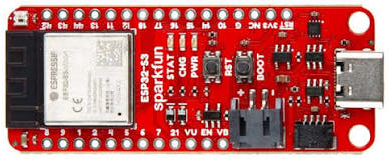
\includegraphics[width=0.6\textwidth]{imagens/sparkfun.jpeg}
	\caption{Placa Arduino Nano ESP32}
\end{figure}

O grande apelo da linha Thing Plus está no design pensado para uso em campo: traz um conector Qwiic (I2C) plug-and-play para encadear sensores sem solda, conector de bateria LiPo com circuito de carga integrado, e suporte a USB-C com funcionalidades USB OTG e Host. Além do processamento veloz com aceleração vetorial para tarefas leves de Inteligência Artificial na borda (Edge AI), a placa expande significativamente o armazenamento disponível. Se destaca pela presença de um slot para cartão microSD acoplado via interface SPI, e permite o armazenamento offline de grande volume de dados de sensores (data logging).

\begin{itemize}
	\item Módulo Principal: ESP32-S3-WROOM-1 (Antena PCB embutida)
	\item Processador Xtensa 32-bit Dual-Core LX7 (até 240 MHz) com extensões vetoriais (IA)
	\item Memória Flash	de 16 MB (Quad SPI Flash)
	\item Memória SRAM / PSRAM de 512 KB SRAM + 8 MB PSRAM (Octal SPI)
	\item Conectividade Sem Fio	Wi-Fi 4 (802.11 b/g/n) + Bluetooth 5 (LE) / Bluetooth Mesh
	\item Conector USB-C (Nativo, com suporte a USB OTG e depuração)
	\item Expansão de Arquivos com slot de cartão MicroSD (Interface SPI)
	\item Ecossistema I2C com conector Qwiic (4 pinos, 3.3V) para rápida conexão de sensores
	\item Gerenciamento de Energia que possui um circuito carregador de bateria LiPo (MCP73831) com conector JST de 2 pinos
\end{itemize}

Essa combinação de conectividade, gerenciamento inteligente de energia por bateria e ecossistema modular faz da SparkFun Thing Plus ESP32-S3 uma plataforma robusta tanto para prototipagem rápida quanto para aplicações finais de automação industrial, monitoramento ambiental e robótica móvel.

\section{Conclusão}
ESP32 simplifica drasticamente o design de circuitos e viabiliza a criação de projetos de automação, robótica e monitoramento ambiental com extrema eficiência energética e suporte a modos de deep sleep. Associada a versatilidade do seu ecossistema de software e a diversidade do hardware. Atende desde desenvolvedores que buscam a velocidade de prototipagem e a simplicidade do Python (MicroPython) até engenheiros que exigem o desempenho, o controle de memória e a multitarefa do C/C++ com FreeRTOS. 

Além disso, a disponibilidade de famílias especializadas — como as séries S para câmeras e IA, C para baixo consumo e arquitetura RISC-V, e H para redes Zigbee e Matter — garante que exista sempre uma variante sob medida para cada requisito técnico e orçamentário. Para projetos alimentados por bateria ou energia solar, ESP32 oferece múltiplos modos de economia de energia. No modo Deep Sleep, desliga a maior parte do chip (mantendo apenas o coprocessador ULP ativo para monitorar sensores) e consome apenas alguns microamperes.

Adquirir e utilizar as placas do ecossistema ESP32 significa investir em uma plataforma moderna, altamente escalável e suportada por uma vasta comunidade global. Seja para montar redes de sensores em agricultura de precisão, criar nós para casas inteligentes ou desenvolver protótipos industriais complexos, essas placas entregam o poder de processamento com a flexibilidade de um microcontrolador, tornando-se a escolha ideal para transformar ideias em soluções funcionais.

Sou um entusiasta do mundo \textbf{Open Source} e novas tecnologias. Qual a diferença entre Livre e Open Source? \underline{Livre} significa que esta apostila é gratuita e pode ser compartilhada a vontade. \underline{Open Source} além de livre todos os arquivos que permitem a geração desta (chamados de arquivos fontes) devem ser disponibilizados para que qualquer pessoa possa modificar ao seu prazer, gerar novas, complementar ou fazer o que quiser. Os fontes da apostila (que foi produzida com o LaTex) está disponibilizado no GitHub \cite{github}. Veja ainda outros artigos que publico sobre tecnologia através do meu Blog Oficial \cite{fernandoanselmo}.

%-----------------------------------------------------------------------------
% REFERÊNCIAS
%-----------------------------------------------------------------------------
\begin{thebibliography}{4}
  	\bibitem{fernandoanselmo} 
	Fernando Anselmo - Blog Oficial de Tecnologia \\
	\url{http://www.fernandoanselmo.blogspot.com.br/}
	
	\bibitem{publicacao} 
	Encontre essa e outras publicações em \\
	\url{https://cetrex.academia.edu/FernandoAnselmo}
	
	\bibitem{github} 
	Repositório para os fontes da apostila \\
	\url{https://github.com/fernandoans/publicacoes}
  
  \bibitem{github} 
  Outro comparativo entre as placas ESP32 \\
  \url{https://esp32.co.uk/esp32-versions-explained-which-board-should-you-buy-2026/}
\end{thebibliography}
  
\end{document}
